\documentclass{beamer}
%
% Choose how your presentation looks.
%
% For more themes, color themes and font themes, see:
% http://deic.uab.es/~iblanes/beamer_gallery/index_by_theme.html
%
\mode<presentation>
{
  \usetheme{Boadilla}      % or try Darmstadt, Madrid, Warsaw, ...
  \usecolortheme{beaver} % or try albatross, beaver, crane, ...
  \usefonttheme{default}  % or try serif, structurebold, ...
  \setbeamertemplate{navigation symbols}{}
  \setbeamertemplate{caption}[numbered]
  
} 

\usepackage{xcolor,colortbl}
\usepackage[english]{babel}
\usepackage[utf8x]{inputenc}
\usepackage{courier}
\usepackage{dsfont}
\usepackage{verbatim} 
\usepackage{enumerate}
\usepackage{tikz}
\usepackage{multirow}
\usepackage{venndiagram}
\usepackage{epigraph} 
%\usepackage{xcolor}

%\usepackage{enumitem}

\usepackage{hyperref}
\hypersetup{
    colorlinks=true,
    linkcolor=blue,
    filecolor=magenta,      
    urlcolor=cyan,
}

\usetikzlibrary{shapes,decorations,arrows,calc,arrows.meta,fit,positioning}
\tikzset{
    -Latex,auto,node distance =1 cm and 1 cm,semithick,
    state/.style ={ellipse, draw, minimum width = 0.7 cm},
    point/.style = {circle, draw, inner sep=0.04cm,fill,node contents={}},
    bidirected/.style={Latex-Latex,dashed},
    el/.style = {inner sep=2pt, align=left, sloped}
}

\setbeamertemplate{enumerate items}[default]

%\setitemize{label=\usebeamerfont*{itemize item}%
%  \usebeamercolor[fg]{itemize item}
%  \usebeamertemplate{itemize item}}

\newcommand{\Mypm}{\mathbin{\tikz [x=1.4ex,y=1.4ex,line width=.1ex] \draw (0.0,0) -- (1.0,0) (0.5,0.08) -- (0.5,0.92) (0.0,0.5) -- (1.0,0.5);}}%

\title[STA-209]{Study Design}
\subtitle{}
\author{Grinnell College}
\date{Fall 2025}

\begin{document}



\begin{frame}
  \titlepage
\end{frame}



\begin{frame}{Review}
We have spent time looking at what we can do with data.
\begin{itemize}
    \item Making graphics + visuals
    \item Describing graphics + visuals
    \item Tables
\end{itemize}
\end{frame}

\begin{frame}{Outline}
Statistics (largely) involves the following three broad domains:
\begin{itemize}
    \item Design -- how do we obtain our data
    \item Description -- graphics and summaries
    \item Inference -- decision-making
\end{itemize} \vspace{8mm}

By the end of today you will be able to answer:
\begin{itemize}
    \item What is the difference between experiments and observational studies?
    \item How do we make \textit{causal} claims? (cause and effect)
    \item How do we avoid \textit{biases} in our data?
\end{itemize}
\end{frame}



\begin{frame}{Review (again)}
\textbf{Population} is a big group of subjects/events/things about which we wish to learn about \vspace{4mm}

\textbf{Parameter} is a \textit{quantifiable} attribute of a population. Most of the time, the parameter value is unknown \vspace{10mm}

\textbf{Sample} is a much smaller, subgroup of a larger population \vspace{4mm}

\textbf{Statistic} is a numerical summary of the sample that we calculate from our sample data
\end{frame}



\begin{frame}{The Statistical Framework}
\begin{center}
\usetikzlibrary{decorations.pathreplacing,positioning, arrows, shapes, calc,shapes.multipart}
\tikzstyle{block1} = [rectangle, draw, fill=yellow!20, 
    text width=10em, text centered, rounded corners, minimum height=6em]
\tikzstyle{block2} = [rectangle, draw, fill=yellow!20, 
    text width=5em, text centered, rounded corners, minimum height=3em]
\tikzset{
    %Define standard arrow tip
    >=stealth,
    % Define arrow style
    pil/.style={
           ->,
           thick,
           shorten <=2pt,
           shorten >=2pt,}
}
\tikzstyle{line} = [draw, -latex]
\begin{tikzpicture}[node distance = 3cm, auto]
            % Place nodes
            \node [block1] (pop) {Population \\ (Parameter)};
            \node [block2, below of=pop] (samp) {Sample \\ (Statistic)};
            
            % Draw edges
            \draw[<-, >=latex, shorten >=2pt, shorten <=2pt, bend right=45, thick]  (pop.west) to node[auto, swap] {Inference}(samp.west);
            \draw[<-, >=latex, shorten >=2pt, shorten <=2pt, bend right=45, thick] (samp.east) to node[auto, swap] {Study Design}(pop.east); 
            
        \end{tikzpicture}
  \end{center}
\end{frame}



\begin{frame}{Anecdotal Evidence}

{\tiny source: IMS Textbook}

1) A man on the news got mercury poisoning from eating swordfish, so the average mercury concentration in swordfish must be dangerously high. \vspace{8mm}


2) I met two students who took more than 7 years to graduate from Duke, so it must take longer
to graduate at Duke than at many other colleges. \vspace{8mm}


3) My friend’s dad had a heart attack and died after they gave him a new heart disease drug, so
the drug must not work.
\end{frame}



\begin{frame}{Types of Studies}
\textbf{Experiments} are studies that involve manipulating a \textit{treatment} that each participant receives
\begin{itemize}
    \item typically treatments are \textit{randomly assigned} to participants
    \item we then measure participants' \textit{response} to the treatment
    \item the treatment is the explanatory variable
\end{itemize} \vspace{8mm}

\textbf{Observational Studies} are studies that do not involve manipulating the explanatory variables for participants. 
\begin{itemize}
    \item we are simply "observing" what is going on without intervening
    \item nearly all surveys are observational studies
\end{itemize}
\end{frame}



\begin{frame}{Types of Studies -- Conclusions}
The type of study affects the conclusions we can draw from data. \vspace{4mm}

\textbf{Experiments}
\begin{itemize}
    \item Good experiments with \textit{random assignment} of treatments can establish a \underline{cause-and-effect} relationship
    \item We need to control everything that could change the response except for the treatments
        \begin{itemize}
            \item randomization of treatments is the best way to accomplish this
        \end{itemize}
\end{itemize} \vspace{4mm}

\textbf{Observational Studies}
\begin{itemize}
    \item No random assignment $\rightarrow$ can't definitively establish cause-and-effect relationships
    \item we are limited to talking about associations only
\end{itemize}
\end{frame}

\begin{frame}{Surveys}
\textbf{Surveys} are a type of observational study where we ask people about their attitudes/opinions/beliefs \vspace{4mm}

Some important things to think about:
\begin{itemize}
    \item How do we select people we talk to?
    \item How many people do we talk to?
    \item How do we obtain information?
        \begin{itemize}
            \item phone, email, in-person?
        \end{itemize}
\end{itemize}
\end{frame}



\begin{frame}{Surveys}
How do we select people? \vspace{6mm}

We want our sample to be \textbf{representative} of our population.
\begin{itemize}
    \item this means that our sample is nearly the same as our population, only smaller
        \begin{itemize}
            \item i.e.: same proportions M/F, same age/ethnic demographics
        \end{itemize}
    \item a representative sample allows us to generalize our results from the sample to the pop.
    \item \textbf{biased}: a sample that is \textbf{not} representative
\end{itemize} \vspace{4mm}

Not always possible to get a representative sample, but this is what we want to strive for
\end{frame}



\begin{frame}{How do we select people?}
\textbf{Random Sample}

We can choose people at random from our population to reduce the chances of getting a biased sample.
\begin{itemize}
    \item usually the best way to get a representative sample
    \item allows us to \textbf{generalize} from our sample to the pop.
\end{itemize} \vspace{8mm}

\textbf{Sample Size (n = ?)}
\begin{itemize}
    \item number of people we survey is important (more people = more info)
    \item sample size is very important, but proportion of pop. surveyed is not
    \item better to have small sample that is representative, than a large sample that is biased
\end{itemize}
\end{frame}



\begin{frame}{How do we select people?}
\textbf{Census} -- Would conducting a census of the entire population be better? \vspace{4mm}

Issues
\begin{itemize}
    \item difficult
    \item time consuming
    \item expensive
\end{itemize}
\end{frame}



\begin{frame}{Sampling Methods}
\textbf{Simple Random Sample (SRS)}
\begin{itemize}
    \item each \underline{combination} of observations has same chance of being selected
    \item if we were to select multiple SRSs again, different observations will be chosen
        \begin{itemize}
            \item variability by sampling $\rightarrow$ sampling variability
        \end{itemize}
\end{itemize} \vspace{6mm}

\begin{columns}

\begin{column}{0.55\textwidth}
\textbf{Stratified Sample}
\begin{itemize}
    \item \textbf{strata}: subgroups of pop., within each the individuals are similar
        \begin{itemize}
            \item individuals within a strata are similar, but strata themselves can be very different
        \end{itemize}
    \item we take a SRS from each strata to ensure each group has representation
\end{itemize}
\centering
\end{column}

  \begin{column}{0.45\textwidth}
\begin{center}
{\tiny geologylearn.blogspot.com/2015/10/rock-layers.html}
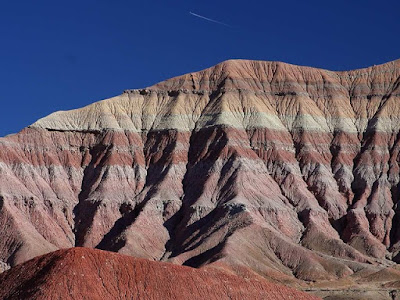
\includegraphics[scale=0.35]{img/strata_rock_layers.jpg}
\end{center}
  \end{column}
\end{columns}
\end{frame}



\begin{frame}{Sampling Example}
Scenario: We want to ask 200 Grinnell students their opinion on if they prefer living in the dorms \vspace{8mm}

\textbf{How do we do this with an SRS?} \vspace{8mm}

\textbf{Why might we want to use a stratified sample?}

\end{frame}



\begin{frame}{Biased Samples}
\textbf{Biased} samples are not representative of the population \vspace{4mm}

\textbf{Voluntary Response Sample}
\begin{itemize}
    \item people select themselves to participate
    \item usually people with strong opinions respond to surveys
\end{itemize} \vspace{4mm}

\textbf{Convenience Sample}
\begin{itemize}
    \item people are chosen in a non-random way
        \begin{itemize}
            \item poll at a specific location
        \end{itemize}
    \item name comes from the fact that this is 'easy' to do
\end{itemize}
\end{frame}



\begin{frame}{Biased Samples}
\textbf{Sampling Bias}
\begin{itemize}
    \item \textbf{undercoverage}: certain groups may not be represented in samples
    \item \textbf{sampling frame} (list of who we can sample from) may be missing some of the population
\end{itemize} \vspace{4mm}

\textbf{Non-response Bias}
\begin{itemize}
    \item some people can't be surveyed or choose not to participate
\end{itemize} \vspace{4mm}

\textbf{Response Bias}
\begin{itemize}
    \item we don't always get accurate info from people
    \item question wording
    \item not wanting to provide truthful answers
\end{itemize}
\end{frame}



\begin{frame}{Intended vs. Actual population}
\begin{center}
    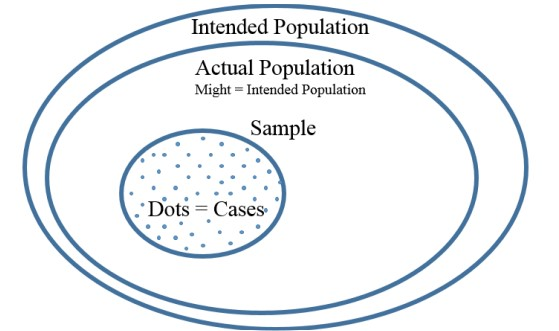
\includegraphics[]{img/actual_intended_pop.jpg}
\end{center}
\text{\tiny source: Dr. Ziegler's Stat 104 notes (ISU)}
\end{frame}


\begin{frame}{Observational Studies}
\textbf{Observational Studies} (again)

Studies where we simply 'observe' what is happening.
\begin{itemize}
    \item we \textbf{can} see associations between variables
    \item we \textbf{cannot} make causal connections between variables
\end{itemize} \vspace{6mm}

Further classification:
\begin{itemize}
    \item \textbf{Prospective study}: pick our sample and collect data as things happen
    \item \textbf{Retrospective study}: look at historical data or past records
\end{itemize}
\end{frame}



\begin{frame}{Experiments}
\textbf{Experiments} (again)
\begin{itemize}
    \item study where researchers manipulate explanatory variables to see effect
    \item explanatory variable values are randomly assigned to each participant
\end{itemize} \vspace{6mm}

\textbf{Experimental Units (EUs)}
\begin{itemize}
    \item the observations (= cases) within our experiment
    \item who/what the experiment is actually performed on
    \item experimental unit = subject = participant
\end{itemize}
\end{frame}


\begin{frame}{Experiments}
\textbf{Factors}
\begin{itemize}
    \item another name for the explanatory variables in the experiment
    \item each experiment must have at least one factor
    \item these are the variables being manipulated for each subject
        \item \textbf{levels} of a factor = values used for that factor
    \begin{itemize}
        \item each factor needs at least two levels
    \end{itemize}
\end{itemize} \vspace{4mm}

\textbf{Treatments}
\begin{itemize}
    \item combo of factors and levels that are given to an EU
    \item one factor $\rightarrow$ levels = treatments
\end{itemize} \vspace{4mm}

\textbf{Response Variables}
\begin{itemize}
    \item EUs' response to a treatment
    \item can have multiple response variables
    \item can be quantitative or categorical (blood pressure vs 'did blood pressure improve')
\end{itemize}
\end{frame}



\begin{frame}{Designing Experiments}
There is much more that goes into designing good experiments. Below are a few commonly used principles. Unfortunately many different principles have the same / similar names. \vspace{4mm}


\textbf{Control} -- 2 types
\begin{itemize}
    \item comparing a treatment to a control group that did not receive the treatment
        \begin{itemize}
            \item treatment vs placebo (or vs 'Gold Standard')
            \item not used in all experiments
        \end{itemize}
    \item control outside sources that might affect response (other variables)
\end{itemize} \vspace{4mm}

\textbf{Replication} -- 2 types
\begin{itemize}
    \item having multiple \textit{replicates} (cases = EUs) for each treatment
    \item \textit{repeatability}: being able to repeat an experiment and get similar results
        \begin{itemize}
            \item same results with a new sample?
            \item do you trust results of a study that we can't confirm on a different sample?
        \end{itemize}
\end{itemize}
\end{frame}



\begin{frame}{Designing Experiments -- Randomness (2 types)}
\textbf{Random Sampling}: picking our sample at random from the population
\begin{itemize}
    \item goal: get sample that is very similar to our population (representative)
    \item allows us to \underline{generalize} our conclusions about the sample to the entire population
\end{itemize} \vspace{4mm}

\textbf{Random Assignment} (randomization): randomly assigning each EU to receive one of the treatments
\begin{itemize}
    \item allows us to make cause-and-effect claims
    \item balances out effect of confounding variables between both groups so that they don't affect our results
    \item results in treatment groups being similar in every regard except for which treatment they receive
\end{itemize}
\end{frame}


\begin{frame}{Experiments -- Randomness}
\begin{center}
    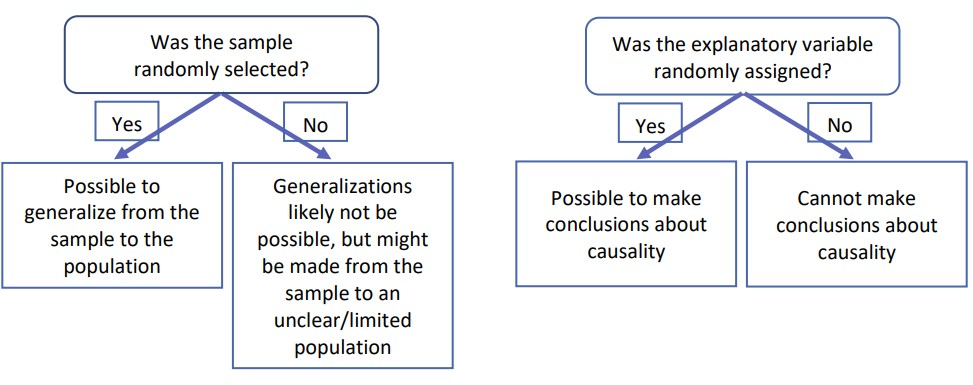
\includegraphics[scale=.7]{img/experiments_conclusions.jpg}
\end{center}
\text{\tiny source: Modified Figure 1.3 from Locke et. al. textbook, Dr. Ziegler (ISU)}
\end{frame}



\begin{frame}{Designing Experiments}
\textbf{Confounding Variable}: a variable that affects our results when we don't want it to
\begin{itemize}
    \item makes it impossible to tell if explanatory variables actually \textbf{caused} changes in response
\end{itemize} \vspace{4mm}

\textbf{How does Randomization fix this issue?}

Random assignment balances a (potentially) confounding variable between the groups $\rightarrow$ it doesn't interfere with out results

\end{frame}



\begin{frame}{Wrapping up -- Reflection}
    What is the difference between an Experiment and an Observational Study? \vspace{4mm}

    Why do Experiments let us make cause-and-effect conclusions? \vspace{4mm}

    What are some ways we can avoid biases when getting our sample? \vspace{4mm}
\end{frame}



\end{document}